% DO NOT COMPILE THIS FILE DIRECTLY!
% This is included by the other .tex files.
\begin{frame}[fragile]
  \frametitle{Overview}
  \begin{itemize}
    \item Upcoming computers
    \item ECP project
    \item exanauts
    \item complex networks
    \item ACOPF (Ipopt and linear solvers)
    \item SCOPF (PIPS and linear solvers)
    \item HiOp (Current-Voltage Rectangular Formulation)
    \item SIMD
    \item 


  \end{itemize}
  \begin{lstlisting}
# some julia code
println( "Here we go with Julia!")
\end{lstlisting}
\end{frame}
\begin{frame}
  \frametitle{Upcoming Supercomputers}
    \begin{center}
      
\includegraphics[width=.25\textwidth]{./figures/ecp} \\
      % \includegraphics[width=.75\textwidth]{./figures/go} 
    \end{center}
  \begin{columns}[T]
    \begin{column}{0.49\textwidth}
      \begin{center}
        {\bf Aurora}\\
        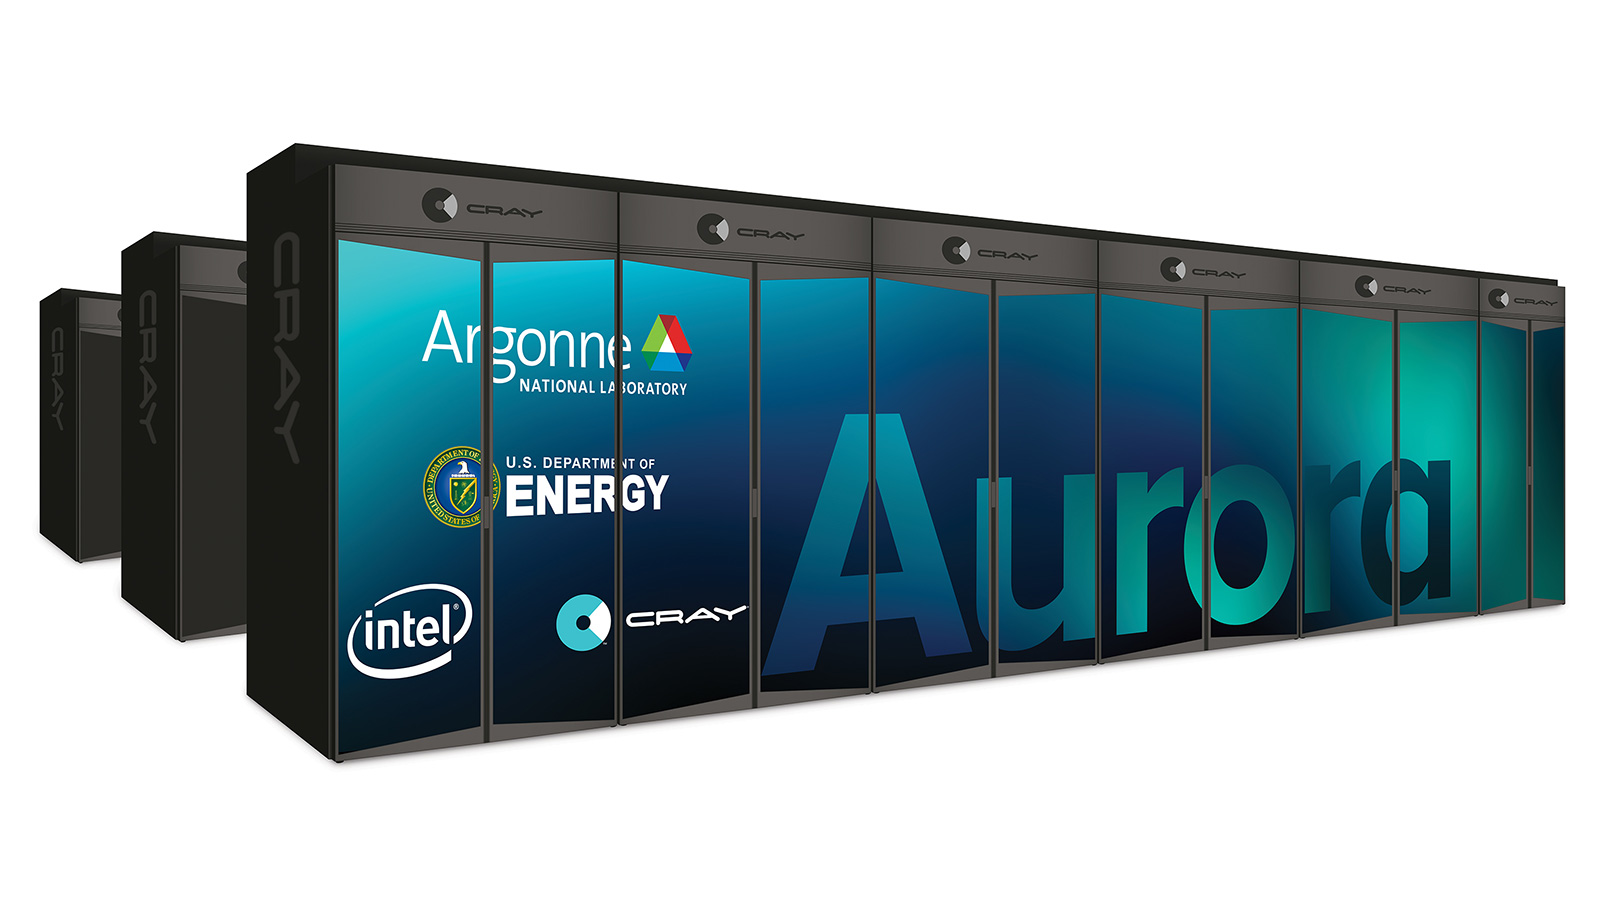
\includegraphics[width=0.75\textwidth]{./figures/aurora}
      \end{center}
    \end{column}
    \begin{column}{0.49\textwidth}
      \begin{center}
        {\bf Frontier}\\
        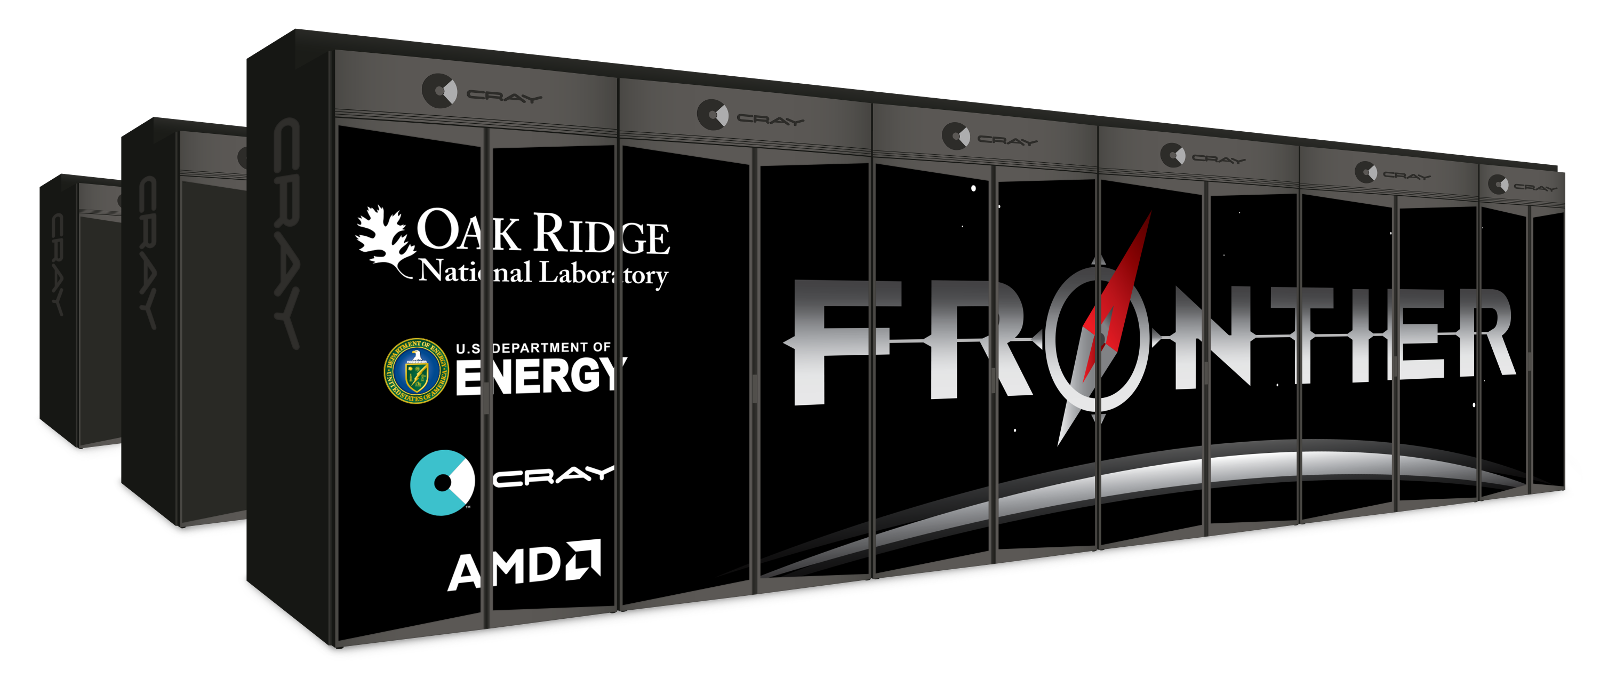
\includegraphics[width=0.75\textwidth]{./figures/frontier}
      \end{center}
    \end{column}
  \end{columns}
  \begin{columns}[T]
    \begin{column}{0.49\textwidth}
    \begin{itemize}
      \item Intel’s Xe compute architecture.
      \item $>$ 1 exaflops
    \end{itemize}
    \end{column}
    \begin{column}{0.49\textwidth}
      \begin{itemize}
        \item AMD EPYC processors and Radeon Instinct GPU
        \item 1.5 exaflops
      \end{itemize}
    \end{column}
  \end{columns}
\end{frame}

\begin{frame}
  \frametitle{Power System}
  \begin{columns}
    \begin{column}{0.45\textwidth}
      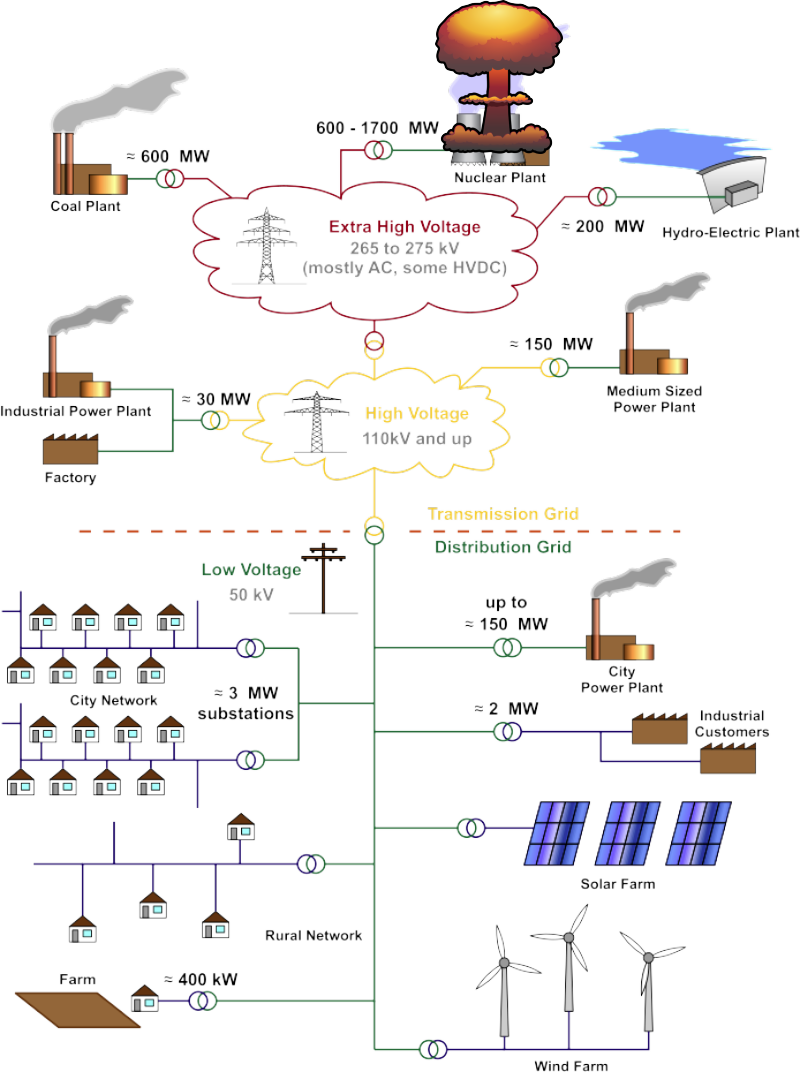
\includegraphics[width=\textwidth]{figures/slides.png}
    \end{column}
    \begin{column}{0.45\textwidth}
      \begin{center}
        % \includegraphics[width=0.8\textwidth]{figures/DampedSine.png}
      \end{center}
      \begin{itemize}
        \item Protect against contingency
        \item Demand is unknown
        \item Generation is unkown (solar, wind, water)
        \item Grid is inherently damped
        \item Steady state, power system dynamics
        \item Reduce outliers, interested in the tails
      \end{itemize}
    \end{column}
  \end{columns}
\end{frame}

\begin{frame}
  \frametitle{ExaSGD: Optimizing Stochastic Grid Dynamics at Exascale
}
\begin{columns}
  \begin{column}{0.45\textwidth}
    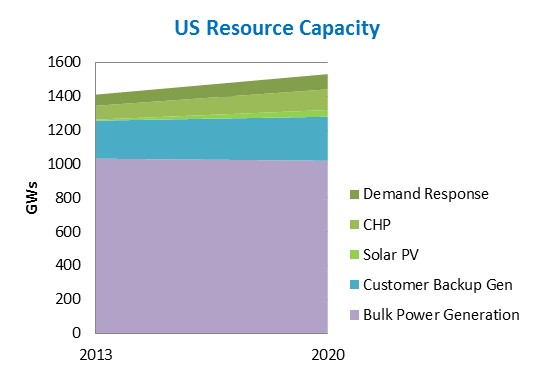
\includegraphics[width=\textwidth]{./figures/generation}
  \end{column}
  \begin{column}{0.45\textwidth}
    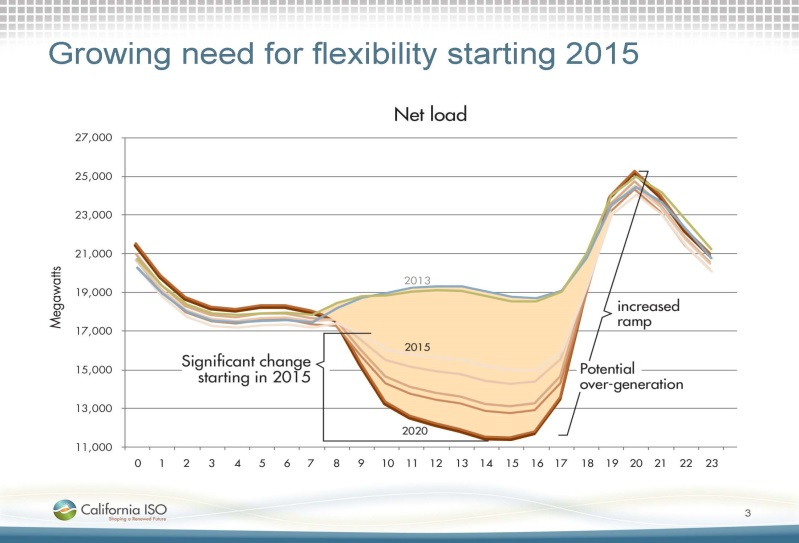
\includegraphics[width=\textwidth]{./figures/ramping}
  \end{column}
\end{columns}
  \begin{center}
      \end{center}
  {\bf Motivation:}
  \begin{itemize}
    \item More renewable energy, more uncertainty
    \item Increase in renewable energy generation ramping
  \end{itemize}
  {\bf Goals:}
  \begin{itemize}
    \item Useful long-term planning model under higher uncertainty
    \item Use AC power flow (nonlinear functions) 
    \item Efficiently leverage exascale hardware in 2021
  \end{itemize}
\end{frame}

\begin{frame}
  \frametitle{Complex Networks}
  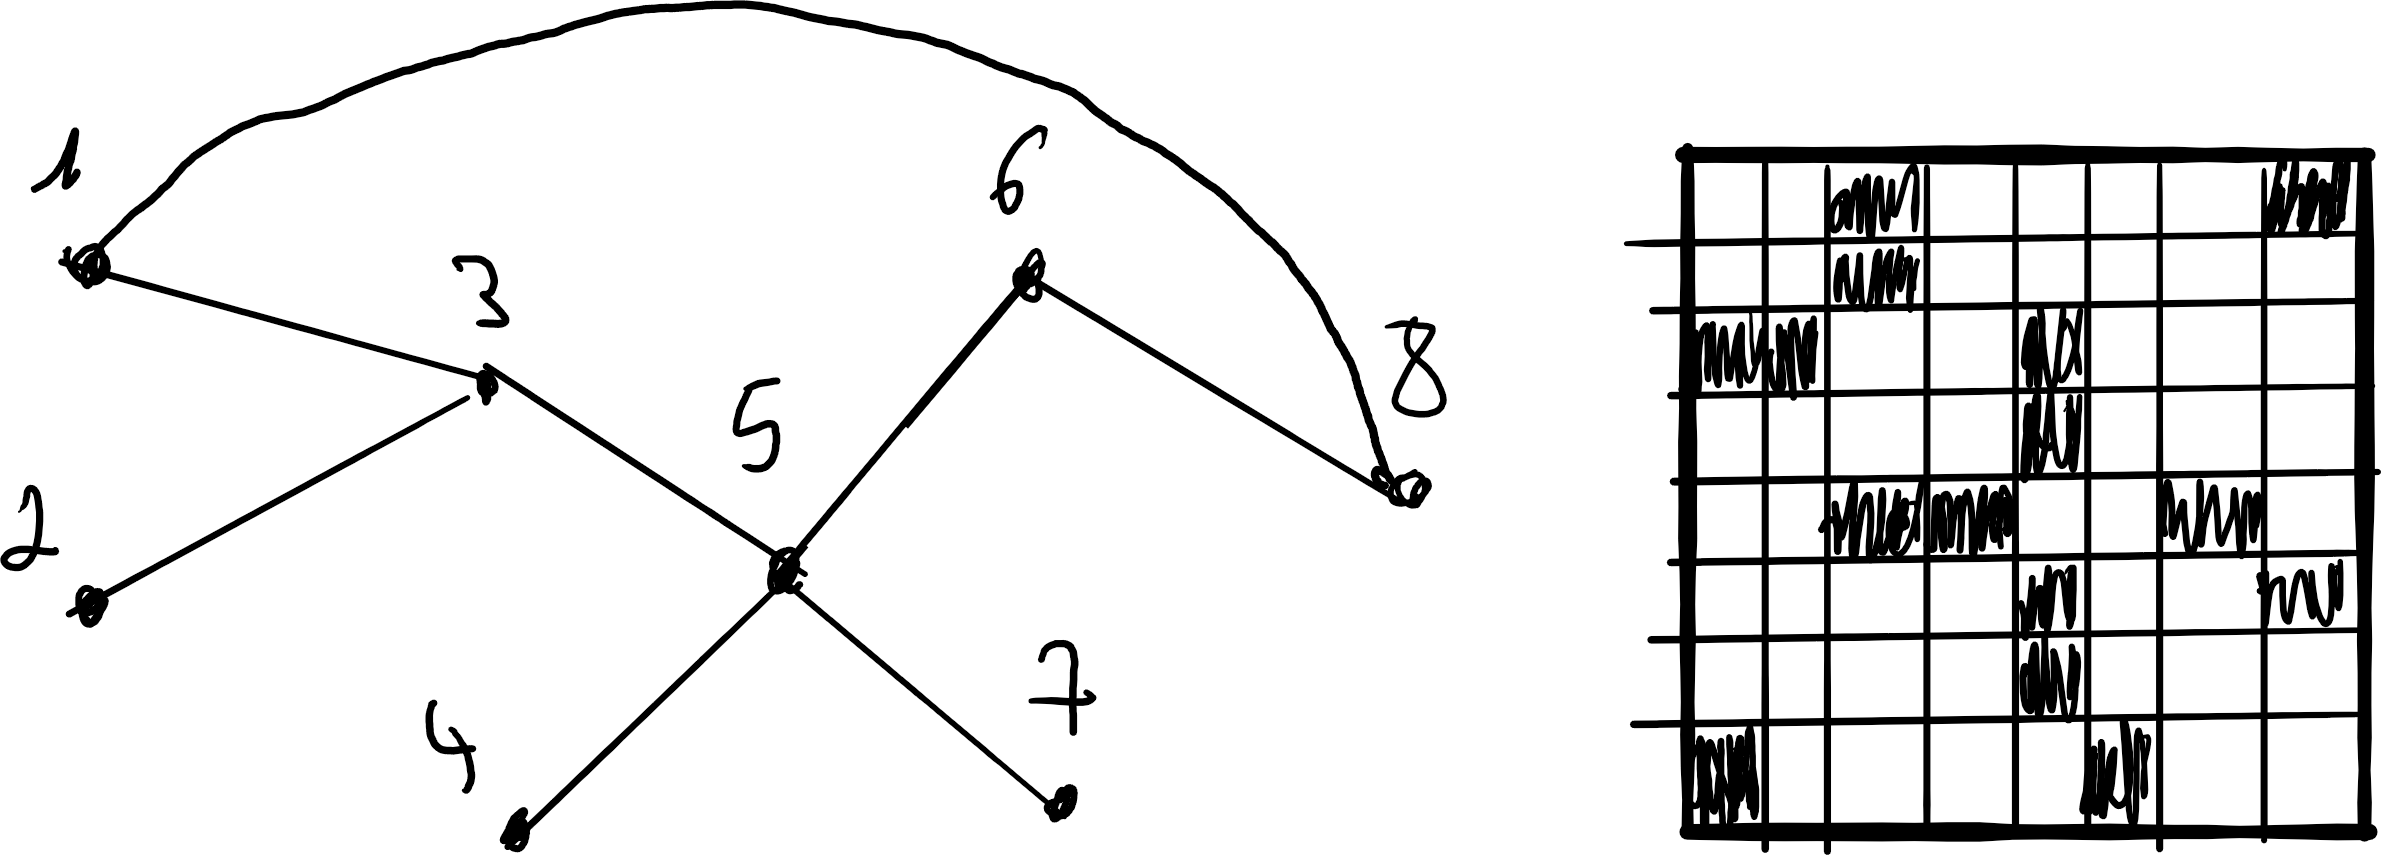
\includegraphics[width=\textwidth]{figures/complexn}
  \begin{itemize}
    \item Examples: Traffic, Internet, power grid
    \item Connection pattern is irregular but not random
    \item Different from most PDE problems (CFD)
    \item Large-scale leads to ill-conditioning
  \end{itemize}
\end{frame}

\begin{frame}[fragile]
  \frametitle{Optimal Power Flow}
  \begin{itemize}
    \item {\bf Objective}
    \begin{itemize}
      \item Generation cost at generators:
      $ \minimize \sum^G_{i=1} c_i(Pg_i)$
    \end{itemize}
    \item {\bf Constraints}
    \begin{itemize}
      \item Kirchhoff's law: What flows in must flow out (nonlinear, non-convex in ACOPF)
      \begin{align*}
        V_k e^{-j\theta_k} & \sum^{N}_{m=0} (G_{km} + jB_{km})V_m e^{j\theta_m} = P - jQ,\ k = 1, \dots, N \\
        \text{where}\\
        V_k &\text{ voltage magnitude at node } k\\
        \theta &\text{ voltage angle at node } k\\
        G_{km} + jB_{km}& \text{ element of nodal admittance matrix}\\
        P, Q &\text{ net real and reactive power entering and leaving node } k
      \end{align*}
      \item Line limits \\
      $$ \theta^{min}_{nm} \leq \theta_n - \theta_m \leq \theta^{max}_{nm}$$
    \end{itemize}
  \end{itemize}
\end{frame}

\begin{frame}[fragile]
  \frametitle{Use Interior-Point for NLP}
  {\bf Solve}
  \begin{align*}
  &\minimize \phi_\mu := f(x)\\ 
  \text{with}&\\
  &g(x) \geq 0, \ i=1,\dots, m \\
  &c(x) = 0, \ j=1,\dots, l \\
  \end{align*}
  {\bf using Newton and barrier functions}
  \begin{align*}
  &\minimize \phi_\mu := f(x) - \mu \sum^m_{i=1} \ln g(x)\\ 
  \text{with}&\\
  &c(x) = 0, \ j=1,\dots, l 
  \end{align*}
  \begin{itemize}
    \item Barrier functions exacerbate ill-conditioning
  \end{itemize}
\end{frame}

\begin{frame}[fragile]
  \frametitle{Interior-Point and GPUs}
  {\bf Current State}
  \begin{itemize}
    \item Very ill-conditioned system (up $1e^{16}$)
    \item Requires sparse direct inertia revealing solver
    \item Ipopt only supports direct solver (exception: Pardiso)
    \item default MUMPS, preferred are HSL libary MA27, MA57 
    \item PIPS-NLP implements Schur complement for two-stage optimization
    \item HiOp mixed dense-sparse solver 
  \end{itemize}
\end{frame}


\begin{frame}[fragile]
  \frametitle{\sout{Optimal} Power Flow}
  \begin{itemize}
    \item {\bf \sout{Objective}}
    \begin{itemize}
      \item \sout{Generation cost at generators:
      $ \minimize \sum^G_{i=1} c_i(Pg_i)$}
    \end{itemize}
    \item {\bf Constraints}
    \begin{itemize}
      \item Kirchhoff's law: What flows in must flow out (nonlinear, non-convex in ACOPF)
      \begin{align*}
        V_k e^{-j\theta_k} & \sum^{N}_{m=0} (G_{km} + jB_{km})V_m e^{j\theta_m} = P - jQ,\ k = 1, \dots, N \\
        \text{where}\\
        V_k &\text{ voltage magnitude at node } k\\
        \theta &\text{ voltage angle at node } k\\
        G_{km} + jB_{km}& \text{ element of nodal admittance matrix}\\
        P, Q &\text{ net real and reactive power entering and leaving node } k
      \end{align*}
      \item \sout{Line limits}\\
      \sout{$ \theta^{min}_{nm} \leq \theta_n - \theta_m \leq \theta^{max}_{nm}$}
    \end{itemize}
  \end{itemize}
\end{frame}

\begin{frame}[fragile]
  \frametitle{Power Flow}
  {\bf Nonlinear equations}
  \begin{itemize}
      \item Kirchhoff's law: What flows in must flow out (nonlinear, non-convex in ACOPF)
      \begin{align*}
        V_k e^{-j\theta_k} & \sum^{N}_{m=0} (G_{km} + jB_{km})V_m e^{j\theta_m} = P - jQ,\ k = 1, \dots, N \\
        \text{where}\\
        V_k &\text{ voltage magnitude at node } k\\
        \theta &\text{ voltage angle at node } k\\
        G_{km} + jB_{km}& \text{ element of nodal admittance matrix}\\
        P, Q &\text{ net real and reactive power entering and leaving node } k
      \end{align*}
      \item Use Newton-Raphson to solve nonlinear equations
  \end{itemize}
\end{frame}

\begin{frame}
  \frametitle{Power Flow}
  {\bf Goal}
  \begin{itemize}
    \item Compute Jacobian using automatic differentiation
    \item Implement a preconditioner
    \item Implement a Krylov method
    \item No computation on the host in main loop, no data transfer
    \item All in Julia, no external calls if possible
  \end{itemize}
\end{frame}

\begin{frame}[fragile]
  \frametitle{Derivatives}
  \begin{center}
  \lstset{linewidth = 0.25\textwidth, frame=tb}
    \begin{lstlisting}
    J\F = dx
    x = x - dx
    \end{lstlisting}
  \end{center}
  \lstset{linewidth = \textwidth}
  {\bf Automatic Differentiation}
  \begin{itemize}
    \item \lstinline{F = f(x)} $\rightarrow$ \lstinline{J = jacobian(x)}
    \item Code transformation
    \item Adjoint \lstinline{adj(x, y) = (J(x))'*y)}, tangent: \lstinline{tgt(x,d) = J(x)*d} 
    \item \lstinline{size(x) >> size(F)} or \lstinline{size(x) << size(F)}
    \item number of buses $\propto$ \lstinline{size(x) = size(F)}
    \item We use \lstinline{ForwardDiff.jl}
  \end{itemize}
\end{frame}

\begin{frame}
  \frametitle{Jacobian Coloring}
  \begin{center}
    \begin{figure}
      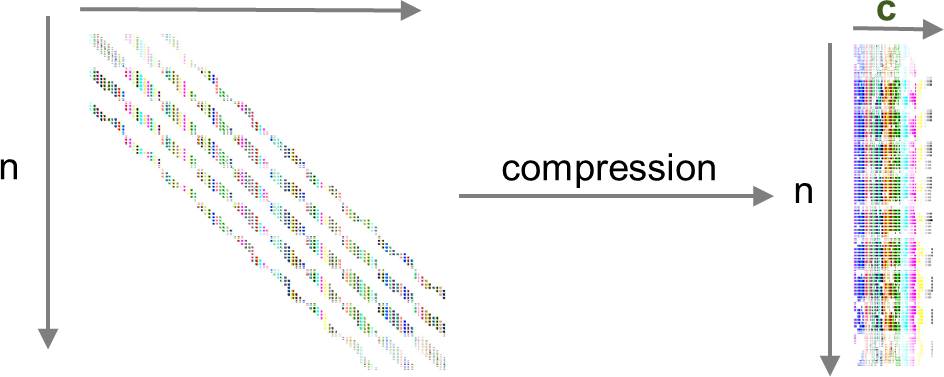
\includegraphics[width=0.65\textwidth]{figures/compression}\footnote{Thanks to Paul Hovland}
      \caption{Jacobian compression}
    \end{figure}
  \end{center}
  \begin{itemize}
    \item Sparse power grid yields very sparse Jacobian
    \item Using greedy algorithm in \lstinline{SparseDiffTools.jl}
  \end{itemize}
\end{frame}

\begin{frame}
  \frametitle{AD on GPUs in Julia}
  \begin{center}
      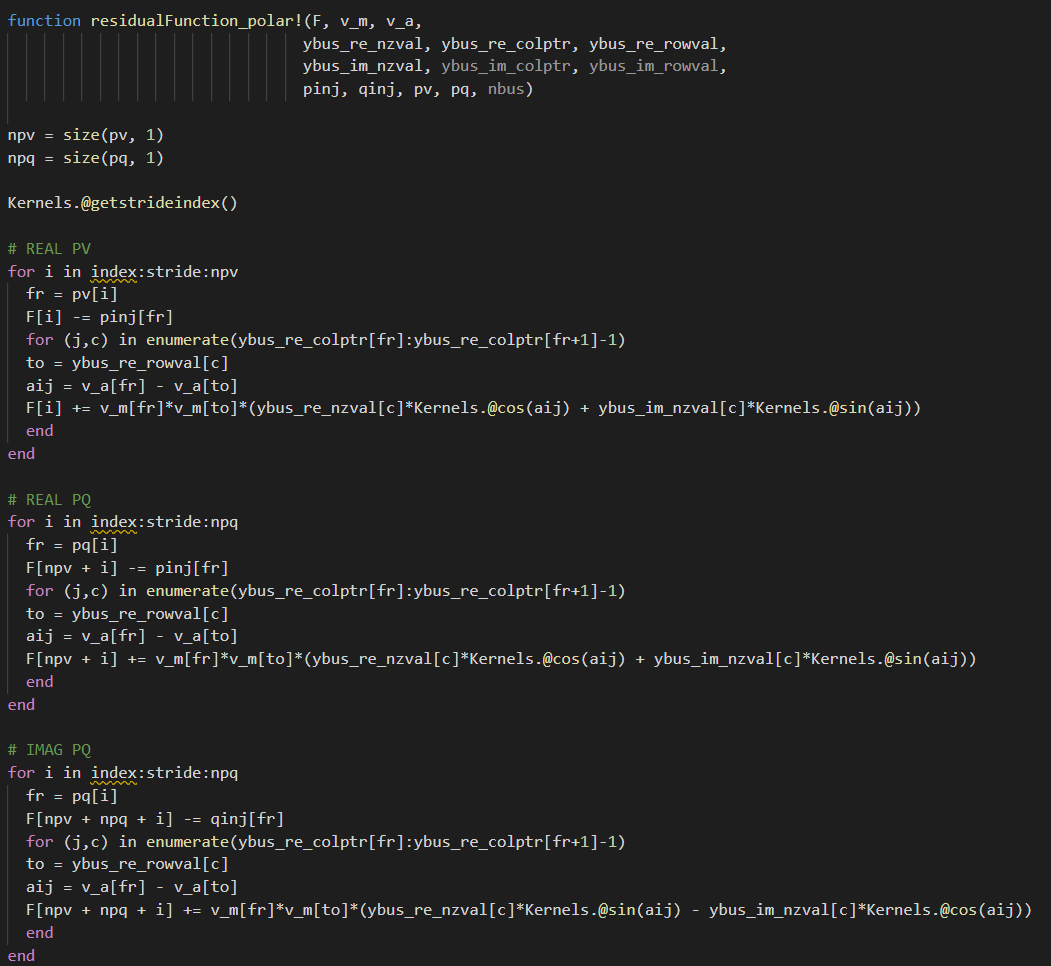
\includegraphics[width=0.55\textwidth]{figures/F}
  \end{center}
\end{frame}
\begin{frame}
  \frametitle{AD on GPUs in Julia}
  \begin{center}
    \lstinline{F = T(undef, n)}
  \end{center}
  \begin{itemize}
    \item Float vector: \lstinline{T = Vector\{Float64\}}
    \item Arbitrary precision vector: \lstinline{T = Vector\{BigFloat\}}
    \item First-order tangent: \lstinline{t1s\{N\} =  ForwardDiff.Dual\{Nothing,Float64, N\} where N}
    \item Second-order tangent: \lstinline{t2s\{M,N\} =  ForwardDiff.Dual\{Nothing,t1s\{N\}, M\} where M, N}
    \item First-order tangent vector: \lstinline{T = Vector\{t1s\{N\}\}}
    \item First-order tangent GPU vector: \lstinline{T = CuVector\{t1s\{N\}\}}
  \end{itemize}
\end{frame}

\begin{frame}
  \frametitle{AD on GPUs in Julia}
  \begin{center}
      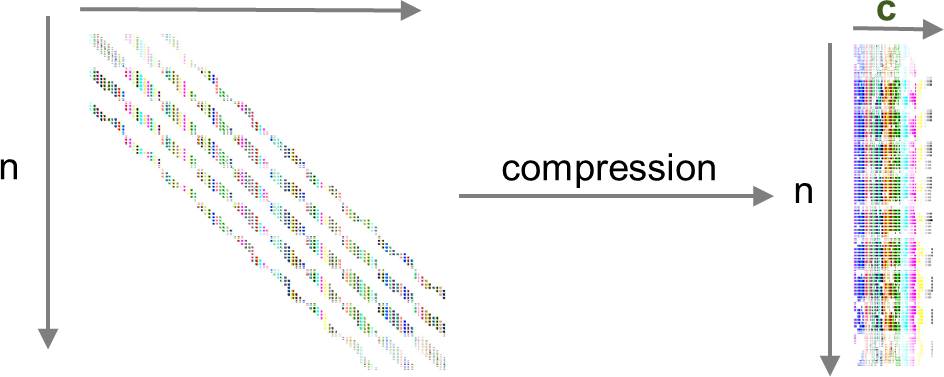
\includegraphics[width=0.45\textwidth]{figures/compression}
      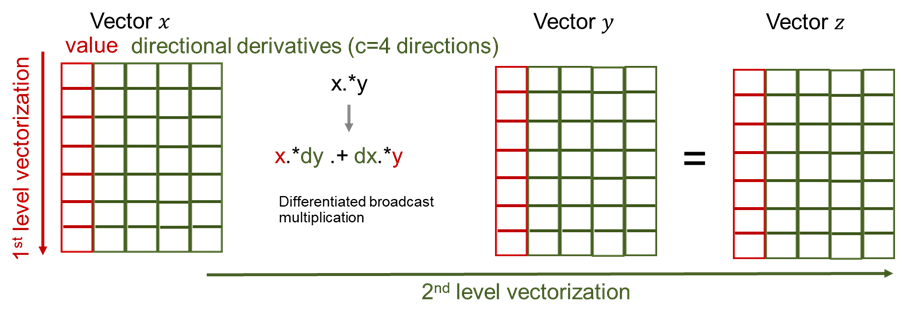
\includegraphics[width=0.55\textwidth]{figures/simd}
  \end{center}
\end{frame}

\begin{frame}
  \frametitle{Jacobian Coloring}
  \begin{center}
    \begin{figure}
      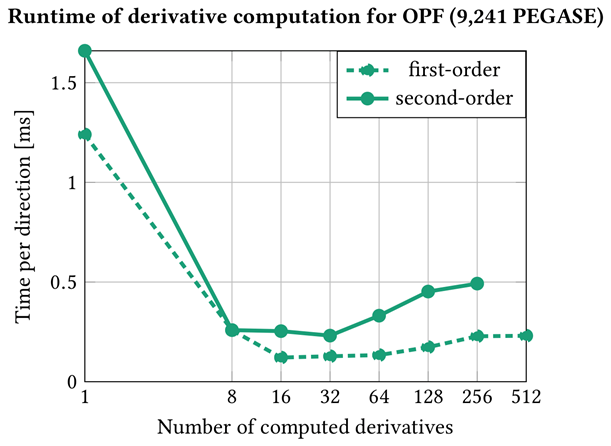
\includegraphics[width=0.35\textwidth]{figures/directionsgpu}
    \end{figure}
  \end{center}
  \begin{itemize}
    \item Sparse power grid yields very sparse Jacobian
    \item Number of colors for 9,241 bus system: 76, Hessian size: 580587x580587, compressed: 580587x76
    \item GPU strategy: Effectively SIMD parallelize over colors/directions
    \item Sweet spot on NVIDIA GV100: Chunks of 32 directions (see Figure)
    \item 0.3ms per color
    \item We don’t expect number colors to exceed 500 for final case
  \end{itemize}
\end{frame}

\begin{frame}
  \frametitle{Preconditioner}
  \begin{center}
    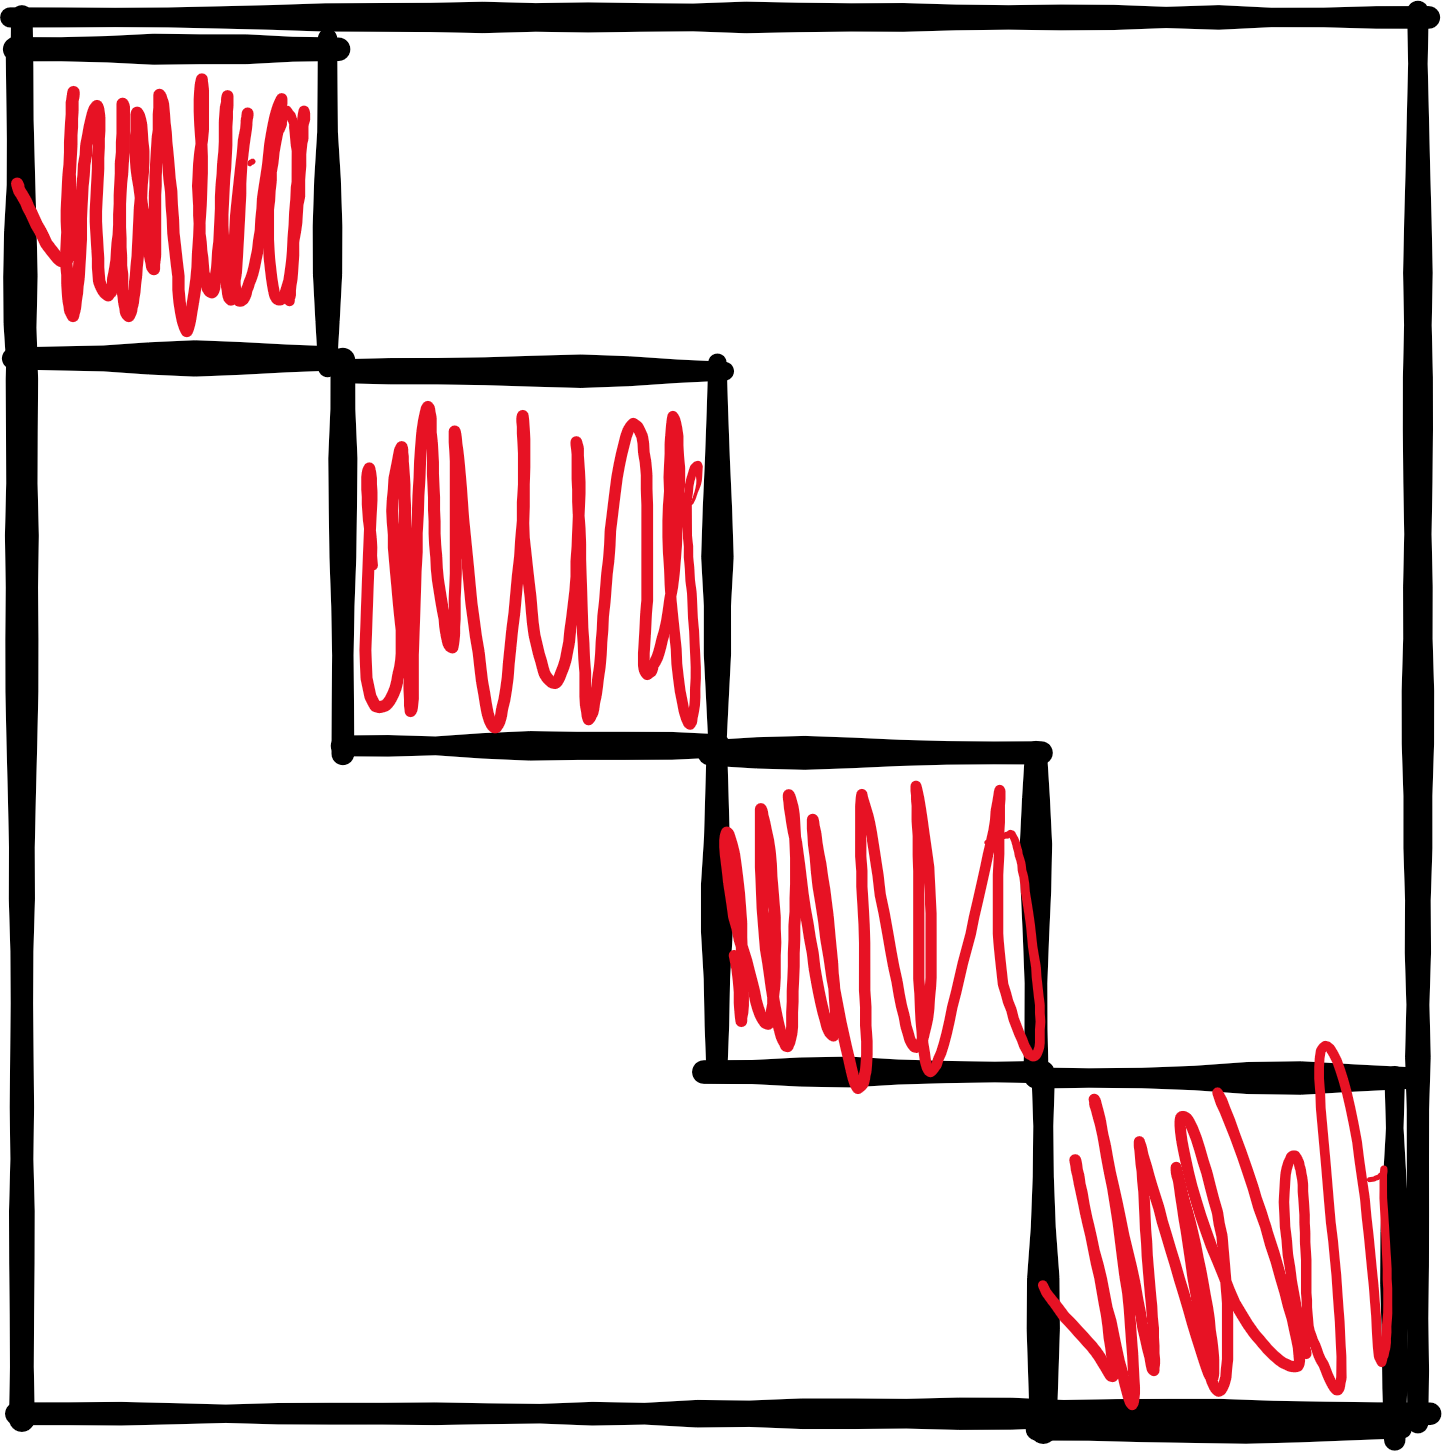
\includegraphics[width=0.25\textwidth]{figures/mpiblocks}
    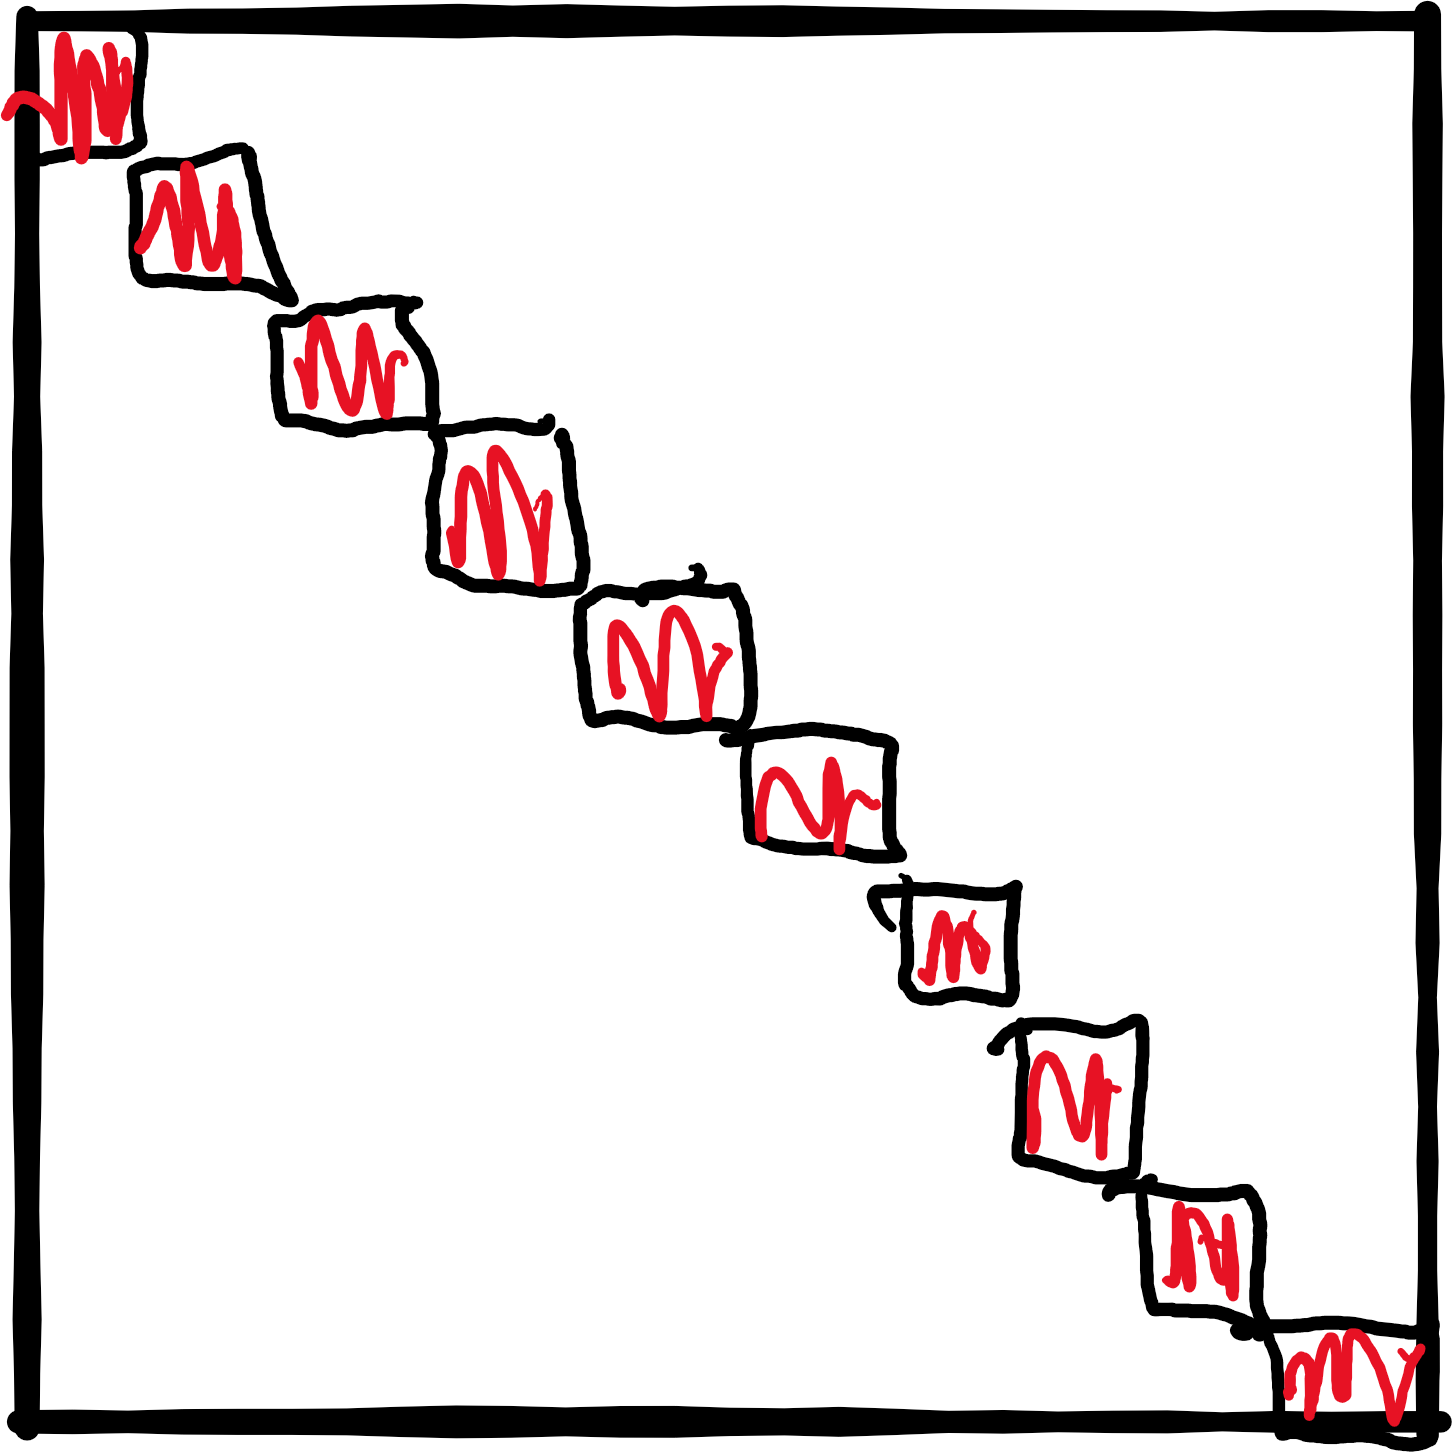
\includegraphics[width=0.25\textwidth]{figures/gpublocks}
  \end{center}
  {\bf Block-Jacobi}
  \begin{itemize}
    \item GPU implementation requires a large number of blocks
    \item PETSc per MPI process: ILU + Krylov \footnote{\cite{schwarz}} 
    \item GPU: Batch CUBLAS LU
    \item Expectation: Increase in number of blocks leads to worse preconditioner
  \end{itemize}
\end{frame}

\begin{frame}
  \frametitle{Preconditioner}
  {\bf Setup}
  \begin{itemize}
    \item Create a partitioning (METIS)
  \end{itemize}
  {\bf Iterate}
  \begin{itemize}
    \item Update P
    \begin{enumerate}
      \item Read dense compressed Jacobian into dense Jacobi blocks
      \item Batch inversion
      \item Update sparse matrix P from dense Jacobi blocks
    \end{enumerate}
  \end{itemize}
  {\bf Code size}
  \begin{itemize}
    \item 200 lines of code for BOTH CPU and GPU implementation
  \end{itemize}
\end{frame}

\begin{frame}
  \frametitle{Preconditioner}
  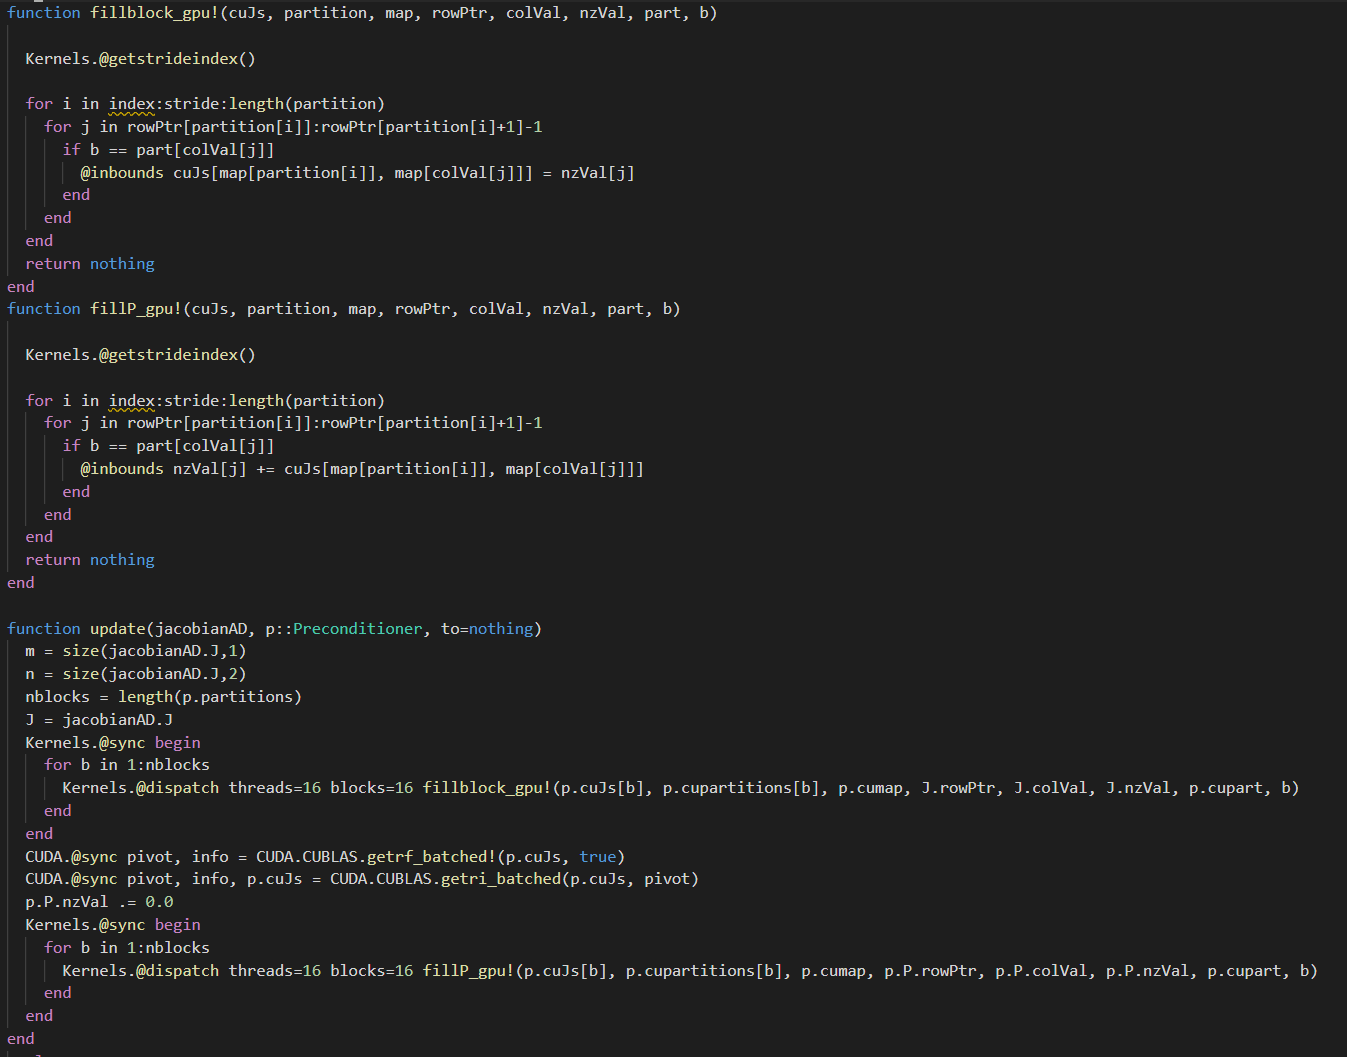
\includegraphics[width=0.95\textwidth]{figures/preconditioner}
\end{frame}

\begin{frame}
  \frametitle{Linear solver}
  {\bf Tour de Solvers}
  \begin{itemize}
    \item Indefinite sparse direct solvers: MA27, MA57, MUMPS, SQPR, CUSOLVER, SPRAL SSIDS
    \item Indefinite dense direct solvers: BLAS, CUBLAS
    \item Sparse positive definite solvers: CHOLMOD, SPRAL SSIDS
    \item Iterative solvers: \lstinline{IterativeSolvers.jl}, \lstinline{Krylov.jl} 
    \item GMRES and BiCGSTAB \footnote{\cite{bicgstabVorst}} \footnote{\cite{sleijpen1993bicgstab}}
  \end{itemize}
\end{frame}

\begin{frame}[fragile]
  \frametitle{Linear Solver}
  \begin{center}
   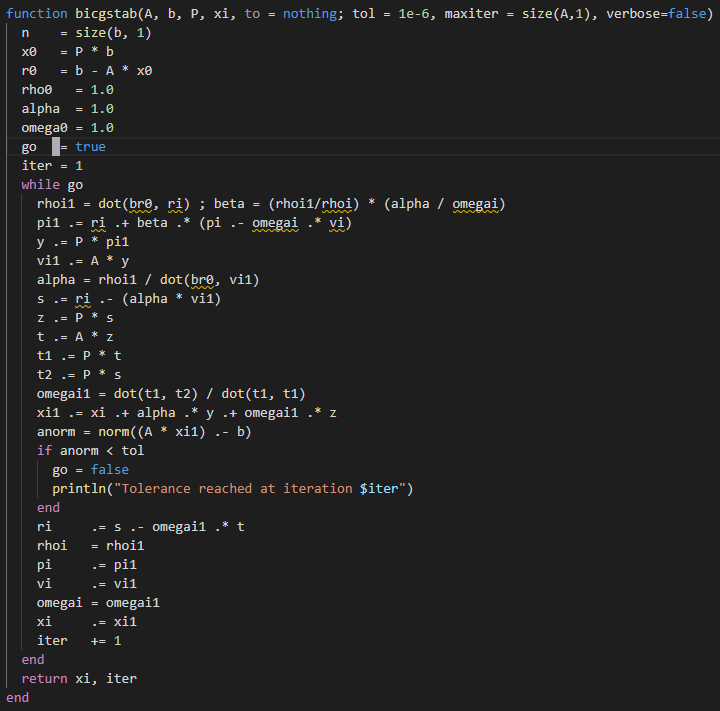
\includegraphics[width=0.7\textwidth]{figures/bicgstab.png}
  \end{center}
\end{frame}

\begin{frame}
  \frametitle{Preconditioner and Linear Solver}
  \begin{center}
   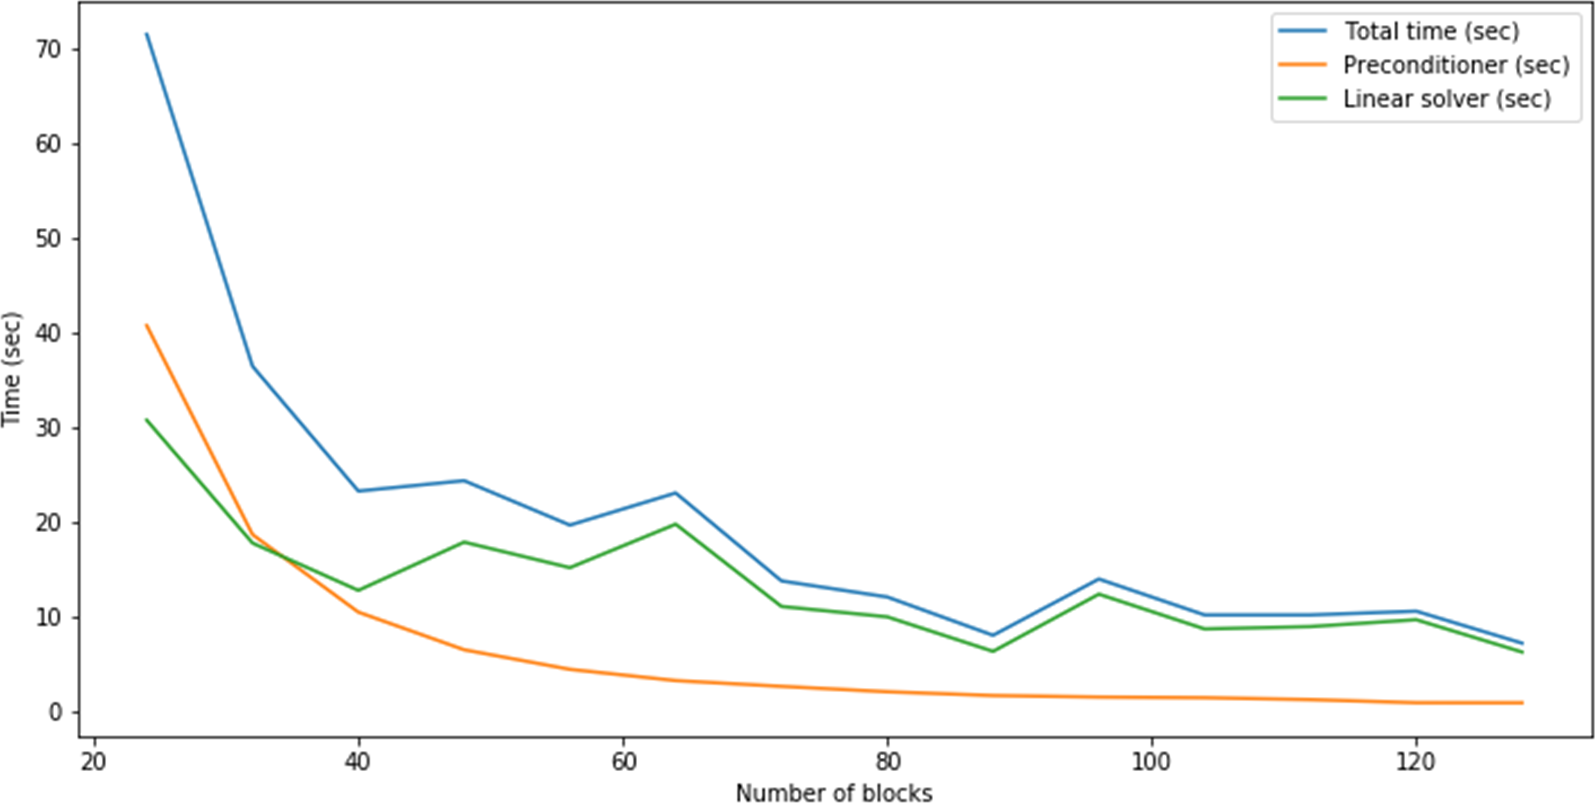
\includegraphics[width=0.45\textwidth]{figures/blocks}
   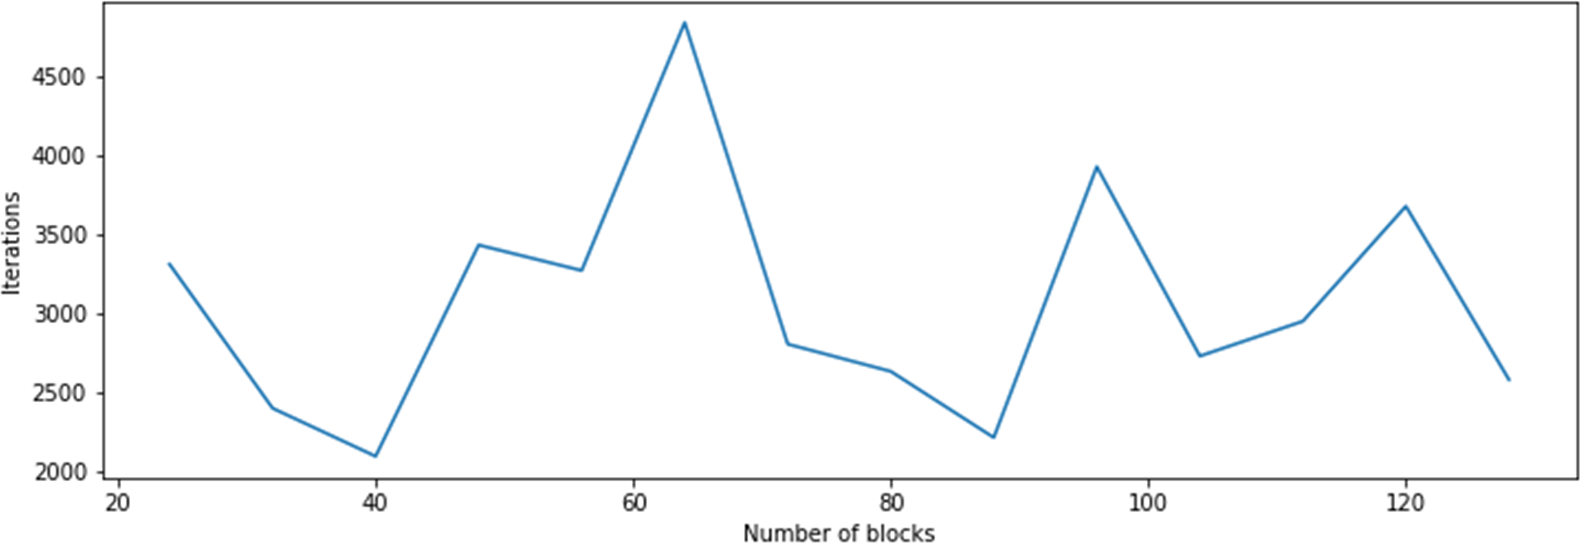
\includegraphics[width=0.45\textwidth]{figures/bicgstabiter}
  \end{center}
  \begin{itemize}
    \item 
  \end{itemize}
\end{frame}

\begin{frame}
  \frametitle{Outlook}
  \begin{itemize}
    \item SIMD modeling framework
    \item Reduced gradient method
  \end{itemize}
\end{frame}



